\section{The operational entanglement}

Consider some $N$-particle quantum state, in which the $N$ particles are shared between spatial subregions $A$ and $B$, or Alice and Bob, if you will. If Alice's and Bob's particles are entangled, this entanglement could be used as a resource for real world applications. Nevertheless, by using the traditional Von Neumann or R\'enyi Entanglement entanglement entropy, an overestimated measure of the physically available entanglement is obtained. This happens because for applications that rely on quantum entanglement, the particle number has to be conserved and these traditional measures do not account for this. To address this issue, Wiseman and Vaccaro \cite{PhysRevLett.91.097902} developed a measure known as Operational Entanglement (originally called Entanglement of Modes by the authors). The operational entanglement takes into account that the local particle number that are in Alice and Bob has to be conserved, giving a more physically accurate measure of entanglement.

	\subsection{Projecting onto subspaces of fixed local particle number}
	
	Knowing the density matrix of subregion $A$ will suffice to calculate, for example, the spatial R\'enyi Entanglement Entropy. Nevertheless, to get the operational entanglement, simply knowing $\rho_{A}$ is not enough. To recap, the spatial R\'enyi Entanglement Entropy is given by:
	

\begin{equation}
 S_{\alpha}(\rho_{A}) = \frac{1}{1-\alpha} \log{\Tr{\rho_{A}^{\alpha}}} 
\end{equation}

Where $\alpha$ is the R\'enyi Index and $\rho_{A}$ is the density matrix of subregion $A$. This calculation is still required to get operational entanglement but, as shall be seen, a few extra steps have to be taken to make sure that local particle number conservation is being satisfied. The first of these extra steps will be to project $\rho_{A}$ to subspaces of local particle number. Projection operators can be written as diagonal matrices with ones on the columns corresponding to the subspace for which the projection is desired. Knowing this, the projection operators into subspaces of fixed local particle numbers can be built rather simply. The projected reduced density matrix of  $A$ into the subspace of fixed local particle number $n$ is obtained by:

\begin{equation}
\rho_{A,n} = \frac{1}{P_n} \hat{\Pi}_n \rho_A \hat{\Pi}_n
\end{equation}

Where $P_n$ is the probability of measuring an Alice state with $n$ particles and $\hat{\Pi}_{n}$ is the projection operator onto the subspace of local particle number $n$.

After all this preamble, the operational entanglement can now be obtained. The operational entanglement is:

\begin{equation}
S_{\alpha}^{op}(\rho_A) = \sum_{n} P_n S(\rho_{A,n}) 
\end{equation}

Where the sum is carried over all possible local particle numbers that Alice may have. In other words, $n=0,1,...,N-n_{B}$.

In the following section, analytical results of the operational entanglement entropy at differential interaction strength regimes in the $tV$ model are derived.


\section{Analytical results at various regimes of the $tV$ model}
	In the $tV$ model, the state of the system is exactly known in three different interaction strength regimes:
	
	\begin{enumerate} [i)]
		%\item Charged Density Wave (CDW): $V/t \to +\infty $
		%\item Phase Separated Solid:  $V/t \to +\infty $
		%\item First Order Phase Transition: V/t = -2
		
		\item$V/t \to +\infty $
		\item $V/t \to +\infty $
		\item $V/t = -2$
	\end{enumerate}
	
	Starting from the known states at these regimes, analytical values for the operational entanglement were calculated. The results will be discussed in this section.

	\subsection{Infinitely repulsive interaction}
		The state in this limit is known as a charged density wave (CDW). In the occupation number basis, the CDW state is:

\[| \Psi \rangle_{CDW} = \frac{1}{\sqrt{2}} [|101010... \rangle + |010101... \rangle ] \]

Where $1$ denotes that the site is occupied and $0$, that it is vacant. The coefficient before the bracket is a normalization constant. As will be shown, the operational entanglement for this state is dependent on the parity of the total number of particles $N$. Up next, the result for even N will be derived.

\begin{samepage}
	\subsubsection{Even N}
	In the following calculations, again, the system will be partitioned into spatial subregions $A$ and $B$, both containing the same number of sites. In other words, if the total number of sites in the $t-V$ chain is $L$, then the partition size will be $l=\frac{L}{2}$. \\
	
In the case of even particle number N, the CDW state will have the same number of particles in each subregion $A$ and $B$:

\begin{equation}
| \Psi \rangle_{N_{Even}} = \frac{1}{\sqrt{2}} [|\underbrace{1010...}_{\frac{N}{2} particles}, \underbrace{1010...}_{\frac{N}{2} particles} \rangle + |\underbrace{0101...}_{\frac{N}{2} particles}, \underbrace{0101...}_{\frac{N}{2} particles} \rangle ] 
\end{equation}

As a reminder, labels left to the comma correspond to spatial subregion $A$, while those to the right correspond to $B$.

The full density matrix $\rho_{AB}$ takes the form:

\begin{equation}
\begin{aligned}
\rho_{AB} &= | \Psi \rangle_{N_{Even}} \langle \Psi |_{N_{Even}} \\
&= \frac{1}{2} |0101...,0101\rangle \langle 0101...,0101... | + \frac{1}{2} |0101...,0101\rangle \langle 1010...,1010... |  \\
&+ \frac{1}{2} |1010...,1010\rangle \langle 0101...,0101... | + \frac{1}{2} |1010...,1010\rangle \langle 1010...,1010... |  \\
\end{aligned}
\end{equation}

Recall that to calculate the entanglement entropies, it is necessary to obtain the reduced density matrix of subsystem $A$. Taking the partial trace with respect to $B$, the reduced density matrix of $A$ is obtained:

\begin{equation}
\begin{aligned}
\rho_{A} &= \Tr_{B} \rho_{AB} &= \sum_{n} {}_B \langle n | \Psi \rangle \langle \Psi | n \rangle_{B} \\
\end{aligned}
\end{equation}

Where the summation is carried over all possible states that $B$ can be found in. In this case, there are only two possible $B$ states: $n = |0101...\rangle_{B}$ and $|1010...\rangle_{B} $Thus, taking the partial trace respect to $B$ of Eq. $(2.5)$:

\begin{equation}
\begin{aligned}
\rho_{A} &= \frac{1}{2} | 0101... \rangle_{A} \langle 0101... |_{A} +  \frac{1}{2} | 1010... \rangle_{A} \langle 1010... |_{A} \\
\end{aligned}
\end{equation}

Notice that some of the terms have vanished due to the orthonormality of the states. At this point, it will be convenient for purposes of illustration to rewrite the reduced density matrix of $A$ in actual matrix form rather than in Dirac or Bra-Ket notation:

\begin{equation}
\begin{aligned}
\rho_{A} &= \begin{pmatrix}
\frac{1}{2} & 0 \\
0 & \frac{1}{2} \\
\end{pmatrix} \\
\end{aligned}
\end{equation}

For spatial entanglement, $\rho_{A}$ would suffice, but for operational entanglement, the matrix has to be projected onto the various subspaces of fixed local particle number in $A$. In this case, both of the states share the same local particle number. That is, the states: $|1010...\rangle_{A}$ and $|0101...\rangle_{A}$ both have local particle number $n = \frac{N}{2}$. Thus only one projection operator is needed. In fact, the operator needed here turns out to be equal to the identity operator:


\begin{equation}
\begin{aligned}
\hat{\Pi}_{n={\frac{N}{2}}} = \begin{pmatrix} 
1&0 \\
0&1 \\
\end{pmatrix} = \hat{I}
\end{aligned}
\end{equation}

The probability of measuring a state with local particle number $n = \frac{N}{2} $ is equal to one. Thus, the projected density matrix of $A$ onto the subspace of $n=\frac{N}{2}$ is:

\begin{align} \rho_{A,\frac{N}{2}} &= \frac{1}{P_{\frac{N}{2}}} \hat{\Pi}_{\frac{N}{2}} \rho_{A} \hat{\Pi}_{\frac{N}{2}} \\ 
& = \hat{I} \rho_{A} \hat{I}  \\
\rho_{A,\frac{N}{2}} &= \rho_{A} = \begin{pmatrix} \frac{1}{2}&0 \\ 0&\frac{1}{2} \end {pmatrix} 
\end{align}

The reduced, projected and normalized reduced density matrix of $A$ is now known and can be substituted into Eq. $2.3$ to calculate the operational entanglement entropy:
\begin {align} 
S_{\alpha}^{op}(\rho_A) &= \sum_{n} P_n S_{\alpha}(\rho_{A,n}) \\
&= \frac{1}{1-\alpha} \log{\Tr{\rho_{A,\frac{N}{2}}^{\alpha}}} \\
&= \frac{1}{1-\alpha} \log{\Tr{\begin{pmatrix}  (\frac{1}{2})^{\alpha} & 0 \\ 0 & (\frac{1}{2})^{\alpha}   \end{pmatrix}}} \\
&= \frac{1}{1-\alpha} \log({\frac{1}{2^{\alpha}} + \frac{1}{2^{\alpha}}}) \\
&= \frac{1}{1-\alpha} \log{2^{(1-\alpha)}} \\
S_{\alpha}^{op}(\rho_A) &= \log{2}
\end {align}

Thus, for even $N$ and $V/t \to + \infty$ , the operational entanglement converges to $\log{2}$. Up next, the result for odd $N$ will be derived.

	\subsubsection{Odd N}
	
	The most general quantum state becomes:
	
	\begin{equation}
	| \Psi \rangle_{N_{Odd}} = \frac{1}{\sqrt{2}} [|\underbrace{...101}_{\frac{N+1}{2} particles}, \underbrace{010...}_{\frac{N-1}{2} particles} \rangle + |\underbrace{...010}_{\frac{N-1}{2} particles}, \underbrace{101...}_{\frac{N+1}{2} particles} \rangle ]
	\end{equation}
	
	Note that now when doing an equal spatial bipartition, one of the subregions will have one more particle than the other, unlike the even particle case in which both subregions had the same number of particles. Specifically, one of the subregions will have $\frac{N+1}{2}$ and the other, $\frac{N-1}{2}$. This implies that $\rho_{A}$ will have to be projected onto the space of local particle number $\frac{N+1}{2}$ and $\frac{N-1}{2}$. But before doing that, again the full body density matrix is needed:
	
	\begin{equation}
	\begin{aligned}
\rho_{AB} &= | \Psi \rangle_{N_{Even}} \langle \Psi |_{N_{Even}} \\
&= \frac{1}{2} |...101,010... \rangle \langle ...101,010... | + \frac{1}{2} |...101,010... \rangle \langle ...010,101... |  \\
&+ \frac{1}{2} |...010,101... \rangle \langle ...101,010... | + \frac{1}{2} |...010,101... \rangle \langle ...010,101... |  \\
	\end{aligned}
	\end{equation}
	
The possible $B$ states are: $n = | 101... \rangle, | 010... \rangle$ with $\frac{N+1}{2}$ and $\frac{N-1}{2}$ particles, respectively. Taking the partial trace respect to B, the reduced density matrix of $A$ becomes:
	
	\begin{equation}
\begin{aligned}
\rho_{A} &= \frac{1}{2} | 101... \rangle_{A} \langle 101... |_{A} +  \frac{1}{2} | 010... \rangle_{A} \langle 010... |_{A} \\
\end{aligned}
\end{equation}

Once again, it may be more illustrative to rewrite in matrix form. Defining an orthonormal basis $| 101... \rangle_{A}  = \begin{pmatrix} 1 \\ 0\end{pmatrix}$ and $| 010... \rangle_{A}  = \begin{pmatrix} 0 \\ 1\end{pmatrix}$ the reduced density matrix of $A$ becomes:

\begin{equation}
\rho_{A} = 
\begin{pmatrix}
\frac{1}{2} & 0 \\
0 & \frac{1}{2}
\end{pmatrix}
\end{equation}

The simple projection operators onto $\frac{N+1}{2}$ and $\frac{N-1}{2}$ particle space in this basis are:

\begin{equation}
\hat{\Pi}_{\frac{N+1}{2}} = \begin{pmatrix} 1 & 0 \\ 0 & 0 \end{pmatrix} , 
\hat{\Pi}_{\frac{N-1}{2}} = \begin{pmatrix} 0 & 0 \\ 0 & 1 \end{pmatrix} 
\end{equation}

Applying these projections to $\rho_{A}$ and choosing the probability such that the trace of each matrix is unity (normalization):

\begin{equation}
\rho_{A,{\frac{N+1}{2}}} = \begin{pmatrix} 1 & 0 \\ 0 & 0 \end{pmatrix}  \text{ with probability } P_{\frac{N+1}{2}} = \frac{1}{2}
\end{equation}

and 

\begin{equation}
\rho_{A,{\frac{N-1}{2}}} = \begin{pmatrix} 0 & 0 \\ 0 & 1 \end{pmatrix}  \text{ with probability } P_{\frac{N-1}{2}} = \frac{1}{2}
\end{equation}

Substituting into the operational entanglement equation (Eq. 2.3):

\begin {align} 
S_{\alpha}^{op}(\rho_A) &= \sum_{n} P_n S_{\alpha}(\rho_{A,n}) \\
&= (\frac{1}{2})\frac{1}{1-\alpha} \log{\Tr{\rho_{A,\frac{N+1}{2}}^{\alpha}}} + (\frac{1}{2})\frac{1}{1-\alpha} \log{\Tr{\rho_{A,\frac{N-1}{2}}^{\alpha}}} \\
&=\frac{1}{2-2\alpha}[ \log{\Tr{\begin{pmatrix}  1^{\alpha} & 0 \\ 0 & 0   \end{pmatrix}}} + \log{\Tr{\begin{pmatrix}  0 & 0 \\ 0 & 1^{\alpha}   \end{pmatrix}}}]\\
&=  \frac{1}{2-2\alpha}[ \underbrace{\log{1} + \log{1}}_{=0} ]\\
S_{\alpha}^{op}(\rho_A) &= 0
\end {align}

Therefore, the operational entanglement vanishes in the infinite repulsion limit ($V/t \to + \infty$) and odd number of particles in the system.

Summarizing:

\begin{equation}
\lim_{V \to + \infty} S_{\alpha}^{op} =
\begin{cases}
\log{2}  & \text{if }N\text{ is even} \\
0 & \text{if }N\text{ is odd}
\end{cases}
\end{equation}

\end{samepage}

	\subsection{Infinitely attractive interaction}
	In this section, an analytical result will be derived at half-filling ($L = 2N$) and partition size equal to the half the number of sites ($\ell = \frac{L}{2}$) for $V/t \to - \infty$. After arriving to the half-filling result, a general result, for any filling fraction and partition size, will be also derived. 
	
	\subsubsection{Half-filling}
	In the infinitely attractive regime of the $tV$ model, $V/t \to -\infty$, the fermions cluster together. The most general state in this regime is:
	
\begin{equation}
\begin{aligned}	
| \Psi \rangle_{PSS} = \frac{1}{\sqrt{L}} [ | \underbrace{111...111}_{N particles} , \underbrace{000...000}_{N vacancies} \rangle + |011...111, 100...000 \rangle + |001...111, 110...000 \rangle  \\
+ ...  + |\underbrace{000...000}_{N vacancies}, \underbrace{111...111}_{N particles} \rangle + |100...000, 011...111 \rangle + ... |111...110, 000...001 \rangle ]
\end{aligned}
\end{equation}

This state is known as a phase separated solid (PSS). There are a total of $L$ possible configurations, hence the normalization constant $\frac{1}{\sqrt{L}}$. 

In an effort to simplify the notation while keeping the calculation general, the $A$ or $B$ states will be relabeled as:

\begin {align*}
&| 111...111 \rangle \to | N \rangle \\
&| 011...111 \rangle \to | N-1 \rangle \\
&| 001...111 \rangle \to | N-2 \rangle \\
&\vdots \\
&| 000...011 \rangle \to | 2 \rangle \\
&| 000...001 \rangle \to | 1 \rangle \\
&| 000...000 \rangle \to | 0 \rangle 
\end {align*}

There is still one flaw with this notation. A $| N-1 \rangle $ state could represent either $| 011...111 \rangle $ or $|111...110 \rangle $. In other words, even though they have the same local particle number $N-1$, the configurations themselves are different. One way in which this problem can be circumvented is by adding a subscript to the label to represent distinct configurations. Since particle number will only be shared between two distinct particle configurations, using subscripts of $1$ and $2$ seems natural. For example: $| 011...111 \rangle \to | (N-1)_1 \rangle$ and $|111...110 \rangle \to | (N-1)_2 \rangle$. $|\Psi\rangle_{PSS}$ now becomes:

\begin{equation}
| \Psi \rangle_{PSS} = \frac{1}{\sqrt{L}} [ |N, 0 \rangle + |(N-1)_1, 1_1 \rangle + |(N-2)_1, 2_1 \rangle  
+ ...  + |0, N \rangle + |1_2, (N-1)_2 \rangle + ... |(N-1)_2, 1_2 \rangle ]
\end{equation}

Taking the outer product of Eq. $2.33$ with itself, the full body density matrix is obtained:

\begin{equation}
\rho_{AB} = | \Psi \rangle_{PSS} \langle \Psi |_{PSS} = 
\begin{pmatrix} 
\frac{1}{L} & \frac{1}{L} & ... & \frac{1}{L} \\
\frac{1}{L} & \frac{1}{L} & ... & \frac{1}{L} \\
\vdots & \vdots & \vdots & \vdots \\
\frac{1}{L} & \frac{1}{L} & ... & \frac{1}{L} \\
\end{pmatrix}
\end{equation}

The full body density matrix is of size $LxL$ with all entries equal to $\frac{1}{L}$. Before proceeding, the basis of this matrix should be described. Columns (from left to right) and rows (from top to bottom) are arranged as: \\ $| N, 0 \rangle , |0, N \rangle , | (N-1)_1, 1_1 \rangle, |(N-1)_2, 1_2 \rangle , | (N-2)_1, 2_1 \rangle , | (N-2)_2, 2_2 \rangle , ... , \\ |2_1, (N-2)_1 \rangle , \rangle, |2_2, (N-2)_2 \rangle , \rangle, |1_1, (N-1)_1 \rangle , \rangle, |1_2, (N-1)_2 \rangle  $ . Notice that configurations that share local particle number have been paired up next to each other. The first two states are exceptions, as their subregions never share the same local particle number with subregions of any other state. Now that the basis has been explained, it's time to get the reduced density matrix of $A$. \\
\\
Taking the partial trace with respect to $B$ of Eq. $2.34$:

\begin{equation}
\rho_{A} = \begin{pmatrix}
\frac{1}{L} & 0 &... & 0 & 0 \\
0 & \frac{1}{L} & ... & 0 & 0 \\
\vdots & \vdots & \ddots & \vdots & \vdots \\
0 & 0 & ... & \frac{1}{L} & 0 \\
0 & 0 & ... & 0 & \frac{1}{L} \\
\end{pmatrix}
\end{equation}

And in the hopes of being as explicit as possible, the rows and columns correspond to the following configurations and in the following order: $| N \rangle , |0 \rangle , | (N-1)_1 \rangle, |(N-1)_2 \rangle , | (N-2)_1 \rangle , | (N-2)_2 \rangle , ... , |2_1 \rangle , |2_2 \rangle , |1_1 \rangle , |1_2 \rangle $ 

Now, $\rho_{A}$ has to be projected onto the subspaces of local particle numbers. The allowed local particle numbers are: $n = N, N-1, N-2 .... 2, 1, 0$. So a total of $\frac{M}{2} + 1$ projections need to be done. There is a projection onto the subspace of $n = 0$, one onto $n = N$ and $\frac{M}{2} -1$ onto the remaining subspaces. The $\frac{M}{2}$ was obtained due to the pairs of states that share local particle number: $|(N-1)_1 \rangle \text{ with } |(N-1)_2 \rangle, |(N-2)_1 \rangle \text{ with } |(N-2)_2 \rangle$ and so on and so forth. The $1$ is subtracted because the pair of states $| 0 \rangle$ and $| N \rangle$ don't share local particle number.

The projection operators for $n=0$ and $n=N$ become:

\begin{equation}
\hat{\Pi}_{N} = \begin{pmatrix} 
1 & 0 &... & 0 & 0 \\
0 & 0 & ... & 0 & 0 \\
\vdots & \vdots & \ddots & \vdots & \vdots \\
0 & 0 & ... & 0 & 0 \\
0 & 0 & ... & 0 & 0 \\
\end{pmatrix} , 
\hat{\Pi}_{0} = \begin{pmatrix} 
0 & 0 &... & 0 & 0 \\
0 & 1 & ... & 0 & 0 \\
\vdots & \vdots & \ddots & \vdots & \vdots \\
0 & 0 & ... & 0 & 0 \\
0 & 0 & ... & 0 & 0 \\
\end{pmatrix}
\end{equation}

For the remaining $\frac{M}{2} - 1$ states, there will be two consecutive non-zero entries in the diagonal. For example:

\begin{equation}
\hat{\Pi}_{N-1} = \begin{pmatrix} 
0 \\
& 0 \\
& & 1 \\
& & & 1 \\
& & & &  0 \\
& & & & & 0 \\
& & & & &  & \ddots \\
& & & & & & &  0 \\
& & & & & & & &  0 \\
\end{pmatrix}
\end{equation}

\begin{equation}
\hat{\Pi}_{N-2} = \begin{pmatrix} 
0 \\
& 0 \\
& & 0 \\
& & & 0 \\
& & & &  1 \\
& & & & & 1 \\
& & & & &  & \ddots \\
& & & & & & &  0 \\
& & & & & & & &  0 \\
\end{pmatrix}
,
\hat{\Pi}_{1} = \begin{pmatrix} 
0 \\
& 0 \\
& & 0 \\
& & & 0 \\
& & & &  0 \\
& & & & & 0 \\
& & & & & & \ddots \\
& & & & & & &  1 \\
& & & & & & & &  1 \\
\end{pmatrix}
\end{equation} \\
\\
Notice from the form of the projection operators that the projected reduced density matrices will be similar to each other but with the two non-zero entries shifted correspondingly in the diagonal. Thus taking the projection onto $n=N-1$ of $\rho_{A}$:

\begin{equation}
\begin{aligned}
\rho_{A,N-1} &= \frac{1}{P_{N-1}} \hat{\Pi}_{N-1} \rho_{A} \hat{\Pi}_{N-1} \\
\rho_{A,N-1} &= \frac{1}{P_{N-1}} \begin{pmatrix} 
0 \\
& 0 \\
& & \frac{1}{L} \\
& & & \frac{1}{L} \\
& & & &  0 \\
& & & & & 0 \\
& & & & &  & \ddots \\
& & & & & & &  0 \\
& & & & & & & &  0 \\
\end{pmatrix} 
\end{aligned}
\end{equation}

The probability of measuring a state with local particle number $N-1$ can be obtained from normalization:

\begin{equation}
\Tr{\rho_{A,N-1}} = 1 \implies \frac{1}{P_{N-1}}\frac{2}{L} = 1 \implies P_{N-1} = \frac{2}{L}
\end{equation}

Thus the projection onto $n=N-1$ of $\rho_{A}$ is:

\begin{equation}
\rho_{A,N-1} = \begin{pmatrix} 
0 \\
& 0 \\
& & \frac{1}{2} \\
& & & \frac{1}{2} \\
& & & &  0 \\
& & & & & 0 \\
& & & & &  & \ddots \\
& & & & & & &  0 \\
& & & & & & & &  0 \\
\end{pmatrix} ; \text{ with probability } P_{N-1} = \frac{2}{L}
\end{equation}

For $n = N-2$:
\begin{equation}
 \rho_{A,N-2} = \begin{pmatrix} 
0 \\
& 0 \\
& & 0  \\
& & & 0 \\
& & & &  \frac{1}{2} \\
& & & & & \frac{1}{2} \\
& & & & &  & \ddots \\
& & & & & & &  0 \\
& & & & & & & &  0 \\
\end{pmatrix} ; \text{ with probability } P_{N-2} = \frac{2}{L}
\end{equation}

and so on and so forth. \\
\\
Similarly, $\rho_{A,N}$ and $\rho_{A,0}$ become:
\begin{equation}
\rho_{A,N} = \begin{pmatrix} 
1 \\
& 0 \\
& & 0  \\
& & & 0 \\
& & & &  0 \\
& & & & & 0 \\
& & & & &  & \ddots \\
& & & & & & &  0 \\
& & & & & & & &  0 \\
\end{pmatrix} ,
\rho_{A,0} = \begin{pmatrix} 
0 \\
& 1 \\
& & 0  \\
& & & 0 \\
& & & &  0 \\
& & & & & 0 \\
& & & & &  & \ddots \\
& & & & & & &  0 \\
& & & & & & & &  0 \\
\end{pmatrix} 
\end{equation}

with probabilities $P_{N} = P_{0} = \frac{1}{L}$

Finally, the operational entanglement is:

\begin{align} 
S_{\alpha}^{op}(\rho_A) &= \sum_{n} P_n S_{\alpha}(\rho_{A,n}) \\
&= \frac{1}{1-\alpha}[\frac{1}{L} \log{\Tr{\rho_{A,N}^\alpha}} + \frac{1}{L} \log{\Tr{\rho_{A,0}^\alpha}} + \frac{2}{L} \log{\Tr{\rho_{A,N-1}^\alpha}}  \\
&+ \frac{2}{L} \log{\Tr{\rho_{A,N-2}^\alpha}} + \dots +\frac{2}{L} \log{\Tr{\rho_{A,2}^\alpha}} + \frac{2}{L} \log{\Tr{\rho_{A,1}^\alpha}} ] \\
&= \frac{1}{L-L\alpha}[ \underbrace{\log{1}}_{=0} +  \underbrace{\log{1}}_{=0} + 2 \log({\frac{1}{2^\alpha}+\frac{1}{2^\alpha}}) \\
&+ 2 \log({\frac{1}{2^\alpha}+\frac{1}{2^\alpha}})+ \dots + 2 \log({\frac{1}{2^\alpha}+\frac{1}{2^\alpha}}) + 2 \log({\frac{1}{2^\alpha}+\frac{1}{2^\alpha}}) ] \\
&= \frac{2}{L-L\alpha}\underbrace{[\log{2^{(1-\alpha)}} + \log{2^{(1-\alpha)}} + \dots + \log{2^{(1-\alpha)}} + \log{2^{(1-\alpha)}}}_{\frac{L}{2} - 1 \text{ terms }}] \\
&= (\frac{L}{2}-1)(\frac{2}{L})\log{2^\frac{1-\alpha}{1-\alpha}} \\
&= (\frac{L-2}{2})(\frac{2}{L})\log{2} ; \text{ recall that } L = 2N \\
S_{\alpha}^{op}(\rho_A) &= \frac{N-1}{N}\log{2}
\end{align}

\subsubsection{Analytical result for any filling fraction and partition size}

The analytical result obtained above for the operational entanglement entropy in the infinitely attractive regime corresponds to the special case of half-filling ($N = \frac{L}{2}$) and equal spatial bipartitions ($\ell_{A} = \ell_{B} = \frac{L}{2}$). Nevertheless, a generalized result can be obtained for ant filling fraction and partition size by counting the number of projected reduced density matrices ($\rho_{A,n}$) that will contribute to the operational entanglement. As it will be shown, the number of contributing matrices will depend on how the quantities $\ell_{A}, \ell_{B}, N \text{ } \&  \text{ }N^{c} = L-N$ relate to each other. Demonstration of the following cases will suffice to get the general result:

\begin{align}
&i) \ell_{A} < N < \ell_{B} \\
&ii) \ell_{B} < N < \ell_{A} \\
&iii)  N < \ell_{A} < \ell_{B} \\
&iv) \ell_{A} < \ell_{B} < N
\end{align}

These four cases actually imply other cases and, in the end, all possible relations between the four parameters should be covered. \\

Case $i)$ $\ell_{A} < N < \ell_{B}$:

The condition here is that the size of the subregion $A$ should be less than the total number of particles $N$ and the size of the subregion $B$ should be greater than both of these quantities. Under such conditions, particle configurations in which $B$ is empty are not possible, since $A$ is too small too fit them all. Two other configurations that will not contribute to the operational entanglement are when $A$ is full ($n_{A} = \ell_{A}$) and when it is empty ($n_{A} = 0$). There is only one possible way of distributing the particles in partition $A$ if it is full and likewise if it is empty. As it was seen in the previous section, then the corresponding projected reduced density matrices $\rho_{A,\ell_{A}}$ and $\rho_{A,0}$ have only one nonzero eigenvalue which, after normalization, becomes 1. Thus, $\ln \rho_{A,\ell_{A}}^{\alpha} = \ln \rho_{A,0}^{\alpha} = 0$. There are a total of $\ell_{A}+1$ possible local particle numbers ($n_{A}$) and since $n_{A} = \ell_{A}$ and $n_{A} = 0$ do not contribute, there are actually $\ell_{A}-1$ contributing projected reduced density matrices. All such projected density matrix will have the form:

\begin{equation}
\rho_{A,n} = \begin{pmatrix} 

\frac{1}{L} & 0 \\
0 & \frac{1}{L} \\

\end{pmatrix}
\end{equation}

The two diagonal elements come from the two configurations that have the same local particle number $n$. Technically, these projected reduced density matrices originally have the same dimensions as those in Eqs.$2.37-2.39,2.41-2.43$. Nevertheless, rows and columns that only have zero entries have been thrown out for compactness. Normalizing:

\begin{equation}
\rho_{A,n} = \frac{1}{P_n} \begin{pmatrix} 

\frac{1}{2} & 0 \\
0 & \frac{1}{2} \\

\end{pmatrix} ; P_n = \frac{2}{L}
\end{equation}

Thus, the operational entanglement becomes:

\begin{equation}
S_{\alpha}^{op} (\ell_A, L) = (\ell_{A} - 1) \frac{2}{L} \ln{2}
\end{equation}

Case $ii)$ $\ell_{B} < N < \ell_{A}$:

This time, partition $B$ is the one that can never be empty. Barring that, the argument is exactly the same as $i)$ and thus:

\begin{equation}
S_{\alpha}^{op} (\ell_{B}, L) = (\ell_{B} - 1) \frac{2}{L} \ln{2}
\end{equation}

Case $iii)$ $N < \ell_{A} < \ell_{B}$:

In contrast to $i)$ and $ii)$, now the particles may all be in $A$ or all in $B$. Nevertheless, in such instances, there is only a single possible configuration of the other partition, that in which it's empty. Thus, the projected reduced density matrices $\rho_{A,N}$ and $\rho_{A,0}$ have only one nonzero eigenvalue and, thus, do not contribute to the operational entanglement. Barring these two, there are then $N-1$ projected reduced density matrices that do contribute. They all have the same form as the ones of $i)$ and $ii)$, that is, $2x2$ diagonal matrices (after throwing out all unnecessary zeroes) with 2 eigenvalues $\frac{1}{2}$ (after normalizing) and probabilities $P_n = \frac{2}{L}$. Thus:

\begin{equation}
S_{\alpha}^{op} (N, L) = (N - 1) \frac{2}{L} \ln{2}
\end{equation}

Case $iv)$ $\ell_{A} < \ell_{B} < N$:

Here, no partition will ever be empty. The maximum allowed particle number in $A$ is going to be $n_{A} = \ell_{A}$ and the smallest one, $n_{A} = N - \ell_{B}$. The partition size of $B$ is subtracted from $N$ because the minimum $n_A$ corresponds to a fully occupied partition $B$, that is $n_B = \ell_B$. The 'leftover' particles on $A$ will hence be the total particle number minus those fully occupying $B$. Notice in all the previous examples that the total number of projected reduced density matrix is equal to the difference between max and min allowed particle number $n_A$ plus 1. That is:

\begin{equation}
\text{Total Projected Reduced Density Matrices} = (n_A)_{max} - (n_A)_{min} + 1
\end{equation}

And for this case,

 \begin{align}
\text{Total Projected Reduced Density Matrices} &= (n_A)_{max} - (n_A)_{min} + 1 \\
&= \ell_A - (N-\ell_B) + 1 \\
&= \underbrace{\ell_A + \ell_B}_{L} - N + 1 \\
\text{Total Projected Reduced Density Matrices} &= L - N + 1
\end{align}

Let $L-N \equiv N^c$. The total number of contributing projected reduced density matrices is:

\begin{align}
\text{Contributing Matrices} &= \text{Total Matrices} - 2 \\
&= (N^c + 1) - 2 \\
\text{Contributing Matrices} &= N^c - 1 \\
\end{align}

the operational entanglement then becomes:

\begin{equation}
S_\alpha^{op}(N^c,L) = (N^c - 1) \frac{2}{L} \ln{2}
\end{equation}

The operational entanglement at the infinitely attractive regime has now been obtained for conditions $i)-iv)$. Notice that it always has the form:

\begin{equation}
S_\alpha^{op}(x,L) = (x - 1) \frac{2}{L} \ln{2}
\end{equation}

where $x$ could be  $\ell_A, \ell_B, N$ or $N^c$. But how to determine which of these variables to choose? Recalling that $L-N = N^c, L-\ell_A = \ell_B$ and $L-\ell_B = \ell_A$, extra inequalities can be obtained from $i)-iv)$ that relate the four variables:

\begin{align}
& i) \ell_{A} < N < \ell_{B} \implies \ell_{B} > N^c > \ell_{A} \implies \ell_{A} \text{ is the smallest} \\
& ii) \ell_{B} < N < \ell_{A} \implies \ell_{A} > N^c > \ell_{B} \implies \ell_{B} \text{ is the smallest} \\
& iii)  N < \ell_{A} < \ell_{B} \implies N^c > \ell_{B} > \ell_{A} \implies N \text{ is the smallest} \\
& iv) \ell_{A} < \ell_{B} < N \implies \ell_{B} > \ell_{A} > N^c \implies N^c \text{ is the smallest} \\
\end{align}

From the above set of inequalities, note that the smallest between the four variables in each case, also happens to be the variable that is substituted for $x$. Thus, in a more compact form, the generalized operational entanglement at the infinitely attractive regime is:

\begin{equation}
S_\alpha^{op}(x,L) = \frac{2(x-1)}{L} \ln{2} ; \text{ where } x = \min{\ell_A, \ell_B, N, N^c}
\end{equation}

	\subsection{First order phase transition}
	
\section{Numerical Results}
	\subsection{Operational entanglement as a function of interaction strength}
		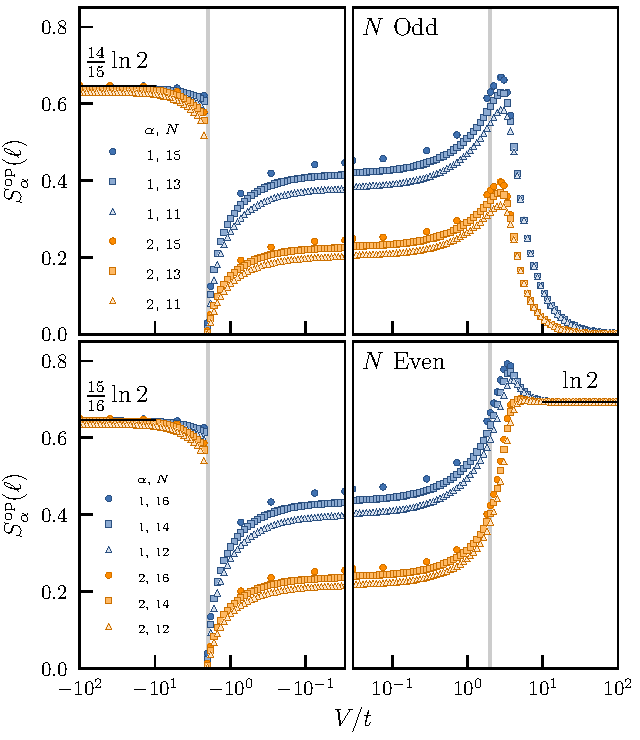
\includegraphics{operationalEntanglementEntropies}
	\subsection{Scaling of operational entanglement peak}
		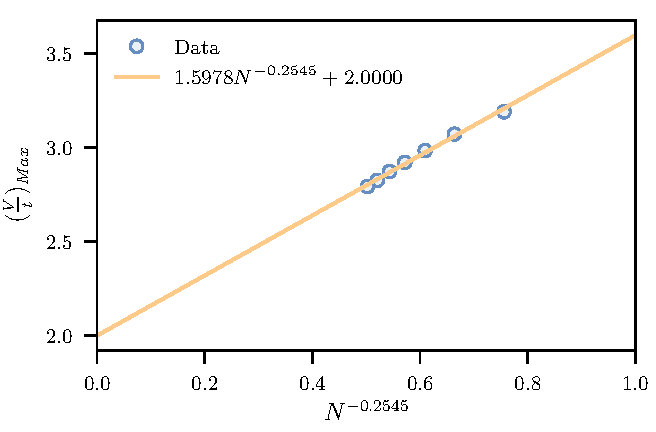
\includegraphics{peakFitOddN_wLegend.pdf}
	\subsection{Entanglement of fluctuations}
	
